% generated by romeo (IRCCyN) : a Tool for Time Petri Nets Analysis  

\documentclass[a4paper,10pt]{article}
\usepackage{tikz} 
 \usetikzlibrary{arrows,automata,positioning,petri}

 
\begin{document}
\begin{figure} 
 {\footnotesize 
 \begin{center}
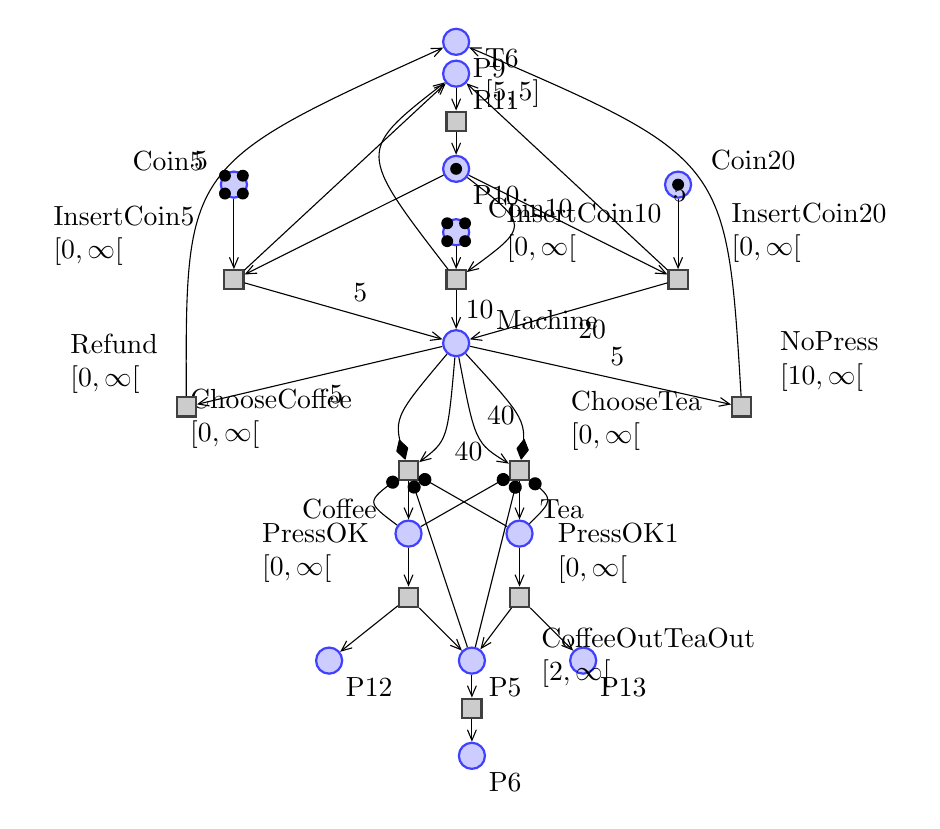
\begin{tikzpicture} 
 [scale =1] 
 \tikzset{node distance =0.7643312101910827cm, bend angle=-45,auto}
\tikzstyle{place}=[circle,thick,draw=blue!75,fill=blue!20,minimum size=7.6 pt]
\tikzstyle{transition}=[rectangle,thick,draw=black!75,fill=black!20,minimum size=6.9 pt]
\node [place,tokens=4](p1) at (160.9 pt,-74.9 pt)[label={[label distance=3.0pt]12.0:Coin10}]{};
\node [place,tokens=0](p2) at (160.9 pt,-115.0 pt)[label={[label distance=5.9pt]8.3:Machine}]{};
\node [place,tokens=0](p3) at (143.7 pt,-183.8 pt)[label={[label distance=3.1pt]166.5:Coffee}]{};
\node [place,tokens=0](p4) at (183.8 pt,-183.8 pt)[label={[label distance=-0.8pt]27.7:Tea}]{};
\node [place,tokens=0](p5) at (166.6 pt,-229.7 pt)[label={[label distance=-1.5pt]-45.0:P5}]{};
\node [place,tokens=0](p6) at (166.6 pt,-264.1 pt)[label={[label distance=-1.5pt]-45.0:P6}]{};
\node [place,tokens=4](p7) at (80.6 pt,-57.7 pt)[label={[label distance=2.5pt]169.5:Coin5}]{};
\node [place,tokens=1](p8) at (241.1 pt,-57.7 pt)[label={[label distance=3.4pt]13.2:Coin20}]{};
\node [place,tokens=0](p9) at (160.9 pt,-6.1 pt)[label={[label distance=-1.5pt]-45.0:P9}]{};
\node [place,tokens=1](p10) at (160.9 pt,-52.0 pt)[label={[label distance=-1.5pt]-45.0:P10}]{};
\node [place,tokens=0](p11) at (160.9 pt,-17.6 pt)[label={[label distance=-1.5pt]-45.0:P11}]{};
\node [place,tokens=0](p12) at (115.0 pt,-229.7 pt)[label={[label distance=-1.5pt]-45.0:P12}]{};
\node [place,tokens=0](p13) at (206.8 pt,-229.7 pt)[label={[label distance=-1.5pt]-45.0:P13}]{};
\node [transition] (t1)  at (160.9 pt,-92.1 pt)[label={[label distance=5.0pt]11.1:\begin{tabular}{l} InsertCoin10 \\  $ [0,\infty[ $ \end{tabular}}]{};
\node [transition] (t1)  at (160.9 pt,-92.1 pt)[label={[text=red,label distance=-6.0pt]45.0:\begin{tabular}{l} $  $ \\  \end{tabular}}]{};
\node [transition] (t1)  at (160.9 pt,-92.1 pt)[label={[text=blue,label distance=-0.7pt]-26.6:\begin{tabular}{l} $  $ \\  \end{tabular}}]{};
\draw[-angle 45] (p1) edge  (t1) ;
\draw[-angle 45] (p10) .. controls (187.6 pt,-72.6 pt) ..  (t1) ;
\draw[-angle 45] (t1) edge node { 10} (p2) ;
\draw[-angle 45] (t1) .. controls (125.0 pt,-45.5 pt) ..  (p11) ;
\node [transition] (t2)  at (143.7 pt,-160.9 pt)[label={[label distance=7.4pt]164.5:\begin{tabular}{l} ChooseCoffee \\  $ [0,\infty[ $ \end{tabular}}]{};
\node [transition] (t2)  at (143.7 pt,-160.9 pt)[label={[text=red,label distance=-6.0pt]45.0:\begin{tabular}{l} $  $ \\  \end{tabular}}]{};
\node [transition] (t2)  at (143.7 pt,-160.9 pt)[label={[text=blue,label distance=-0.7pt]-26.6:\begin{tabular}{l} $  $ \\  \end{tabular}}]{};
\draw[-angle 45] (p2) .. controls (157.8 pt,-150.2 pt) .. node { 40} (t2) ;
\draw[-*] (p3) .. controls (128.4 pt,-172.4 pt) ..  (t2) ;
\draw[-diamond] (p2) .. controls (138.0 pt,-142.2 pt) ..  (t2) ;
\draw[-*] (p5) edge  (t2) ;
\draw[-*] (p4) edge  (t2) ;
\draw[-angle 45] (t2) edge  (p3) ;
\node [transition] (t3)  at (183.8 pt,-160.9 pt)[label={[label distance=5.4pt]15.0:\begin{tabular}{l} ChooseTea \\  $ [0,\infty[ $ \end{tabular}}]{};
\node [transition] (t3)  at (183.8 pt,-160.9 pt)[label={[text=red,label distance=-6.0pt]45.0:\begin{tabular}{l} $  $ \\  \end{tabular}}]{};
\node [transition] (t3)  at (183.8 pt,-160.9 pt)[label={[text=blue,label distance=-0.7pt]-26.6:\begin{tabular}{l} $  $ \\  \end{tabular}}]{};
\draw[-angle 45] (p2) .. controls (167.8 pt,-151.0 pt) .. node { 40} (t3) ;
\draw[-*] (p4) .. controls (196.1 pt,-171.6 pt) ..  (t3) ;
\draw[-diamond] (p2) .. controls (186.5 pt,-142.9 pt) ..  (t3) ;
\draw[-*] (p5) edge  (t3) ;
\draw[-*] (p3) edge  (t3) ;
\draw[-angle 45] (t3) edge  (p4) ;
\node [transition] (t4)  at (143.7 pt,-206.8 pt)[label={[label distance=0.9pt]173.9:\begin{tabular}{l} PressOK \\  $ [0,\infty[ $ \end{tabular}}]{};
\node [transition] (t4)  at (143.7 pt,-206.8 pt)[label={[text=red,label distance=-6.0pt]45.0:\begin{tabular}{l} $  $ \\  \end{tabular}}]{};
\node [transition] (t4)  at (143.7 pt,-206.8 pt)[label={[text=blue,label distance=-0.7pt]-26.6:\begin{tabular}{l} $  $ \\  \end{tabular}}]{};
\draw[-angle 45] (p3) edge  (t4) ;
\draw[-angle 45] (t4) edge  (p5) ;
\draw[-angle 45] (t4) edge  (p12) ;
\node [transition] (t5)  at (183.8 pt,-206.8 pt)[label={[label distance=0.5pt]7.6:\begin{tabular}{l} PressOK1 \\  $ [0,\infty[ $ \end{tabular}}]{};
\node [transition] (t5)  at (183.8 pt,-206.8 pt)[label={[text=red,label distance=-6.0pt]45.0:\begin{tabular}{l} $  $ \\  \end{tabular}}]{};
\node [transition] (t5)  at (183.8 pt,-206.8 pt)[label={[text=blue,label distance=-0.7pt]-26.6:\begin{tabular}{l} $  $ \\  \end{tabular}}]{};
\draw[-angle 45] (p4) edge  (t5) ;
\draw[-angle 45] (t5) edge  (p5) ;
\draw[-angle 45] (t5) edge  (p13) ;
\node [transition] (t6)  at (160.9 pt,-34.8 pt)[label={[label distance=-3.2pt]21.5:\begin{tabular}{l} T6 \\  $ [5,5] $ \end{tabular}}]{};
\node [transition] (t6)  at (160.9 pt,-34.8 pt)[label={[text=red,label distance=-6.0pt]45.0:\begin{tabular}{l} $  $ \\  \end{tabular}}]{};
\node [transition] (t6)  at (160.9 pt,-34.8 pt)[label={[text=blue,label distance=-0.7pt]-26.6:\begin{tabular}{l} $  $ \\  \end{tabular}}]{};
\draw[-angle 45] (p11) edge  (t6) ;
\draw[-angle 45] (t6) edge  (p10) ;
\node [transition] (t7)  at (166.6 pt,-246.9 pt)[label={[label distance=11.9pt]10.0:\begin{tabular}{l} CoffeeOutTeaOut \\  $ [2,\infty[ $ \end{tabular}}]{};
\node [transition] (t7)  at (166.6 pt,-246.9 pt)[label={[text=red,label distance=-6.0pt]45.0:\begin{tabular}{l} $  $ \\  \end{tabular}}]{};
\node [transition] (t7)  at (166.6 pt,-246.9 pt)[label={[text=blue,label distance=-0.7pt]-26.6:\begin{tabular}{l} $  $ \\  \end{tabular}}]{};
\draw[-angle 45] (p5) edge  (t7) ;
\draw[-angle 45] (t7) edge  (p6) ;
\node [transition] (t9)  at (63.4 pt,-138.0 pt)[label={[label distance=-3.1pt]167.2:\begin{tabular}{l} Refund \\  $ [0,\infty[ $ \end{tabular}}]{};
\node [transition] (t9)  at (63.4 pt,-138.0 pt)[label={[text=red,label distance=-6.0pt]45.0:\begin{tabular}{l} $  $ \\  \end{tabular}}]{};
\node [transition] (t9)  at (63.4 pt,-138.0 pt)[label={[text=blue,label distance=-0.7pt]-26.6:\begin{tabular}{l} $  $ \\  \end{tabular}}]{};
\draw[-angle 45] (p2) edge node { 5} (t9) ;
\draw[-angle 45] (t9) .. controls (63.1 pt,-50.4 pt) .. node { 5} (p9) ;
\node [transition] (t10)  at (264.1 pt,-138.0 pt)[label={[label distance=0.5pt]14.0:\begin{tabular}{l} NoPress \\  $ [10,\infty[ $ \end{tabular}}]{};
\node [transition] (t10)  at (264.1 pt,-138.0 pt)[label={[text=red,label distance=-6.0pt]45.0:\begin{tabular}{l} $  $ \\  \end{tabular}}]{};
\node [transition] (t10)  at (264.1 pt,-138.0 pt)[label={[text=blue,label distance=-0.7pt]-26.6:\begin{tabular}{l} $  $ \\  \end{tabular}}]{};
\draw[-angle 45] (p2) edge node { 5} (t10) ;
\draw[-angle 45] (t10) .. controls (258.7 pt,-48.2 pt) .. node { 5} (p9) ;
\node [transition] (t12)  at (80.6 pt,-92.1 pt)[label={[label distance=0.9pt]172.7:\begin{tabular}{l} InsertCoin5 \\  $ [0,\infty[ $ \end{tabular}}]{};
\node [transition] (t12)  at (80.6 pt,-92.1 pt)[label={[text=red,label distance=-6.0pt]45.0:\begin{tabular}{l} $  $ \\  \end{tabular}}]{};
\node [transition] (t12)  at (80.6 pt,-92.1 pt)[label={[text=blue,label distance=-0.7pt]-26.6:\begin{tabular}{l} $  $ \\  \end{tabular}}]{};
\draw[-angle 45] (p7) edge  (t12) ;
\draw[-angle 45] (p10) edge  (t12) ;
\draw[-angle 45] (t12) edge node { 5} (p2) ;
\draw[-angle 45] (t12) edge  (p11) ;
\node [transition] (t13)  at (241.1 pt,-92.1 pt)[label={[label distance=6.1pt]10.6:\begin{tabular}{l} InsertCoin20 \\  $ [0,\infty[ $ \end{tabular}}]{};
\node [transition] (t13)  at (241.1 pt,-92.1 pt)[label={[text=red,label distance=-6.0pt]45.0:\begin{tabular}{l} $  $ \\  \end{tabular}}]{};
\node [transition] (t13)  at (241.1 pt,-92.1 pt)[label={[text=blue,label distance=-0.7pt]-26.6:\begin{tabular}{l} $  $ \\  \end{tabular}}]{};
\draw[-angle 45] (p8) edge  (t13) ;
\draw[-angle 45] (p10) edge  (t13) ;
\draw[-angle 45] (t13) edge node { 20} (p2) ;
\draw[-angle 45] (t13) edge  (p11) ;
\end{tikzpicture} 
 \end{center} 
 } 
 
 \end{figure}

 
\end{document}
